%
%   This file is part of the APS files in the REVTeX 4.1 distribution.
%   Version 4.1r of REVTeX, August 2010
%
%   Copyright (c) 2009, 2010 The American Physical Society.
%
%   See the REVTeX 4 README file for restrictions and more information.
%
\documentclass[%
 reprint,
%superscriptaddress,
%groupedaddress,
%unsortedaddress,
%runinaddress,
%frontmatterverbose, 
% preprint,
%showpacs,preprintnumbers,
%nofootinbib,
%nobibnotes,
%bibnotes,
 amsmath,amssymb,
 aps,
 pra,
%prb,
%rmp,
%prstab,
%prstper,
%floatfix,
]{revtex4-1}

%%%%%%%%%%%%%%%%%%%%%%%%%%%%%%%%%%%%%%%%%%%%%
% IMPORTS
\usepackage{graphicx}          % Include figure files
\usepackage{dcolumn}           % Align table columns on decimal point
\usepackage{bm}                % bold math
% \usepackage{hyperref}          % add hypertext capabilities
% \usepackage[mathlines]{lineno} % Enable numbering of text and display math
% \linenumbers\relax             % Commence numbering lines

\usepackage{lmodern}           % Font package

% Non-standard geometry import
%\usepackage[showframe,%Uncomment any one of the following lines to test 
%%scale=0.7, marginratio={1:1, 2:3}, ignoreall,% default settings
%%text={7in,10in},centering,
%%margin=1.5in,
%%total={6.5in,8.75in}, top=1.2in, left=0.9in, includefoot,
%%height=10in,a5paper,hmargin={3cm,0.8in},
%]{geometry}

%%%%%%%%%%%%%%%%%%%%%%%%%%%%%%%%%%%%%%%%%%%%%
% COMMANDS
\newcommand{\D}{\mathrm{d}}
\newcommand{\iu}{{i\mkern1mu}}

\begin{document}
{\fontfamily{lmss}\selectfont

\preprint{APS/123-QED}

\title{Telescope Diffraction}

\author{Patrick Anker}
\author{Kaitlyn Morrell}
\affiliation{%
 New York University
}

\date{November 17, 2017}

\begin{abstract}
%Abstract *rough* draft
The wave nature of light gives rise to phenomena such as interference and diffraction. These are observed in the application of optics to telescopes. To explore the various effects that result from different telescope designs, we employ two-dimensional Fourier analysis and simulate environmental factors using Gaussian random fields. Additionally, we investigate the results for different power spectrum inputs and examine the effects on the point spread function.
\end{abstract}

\maketitle

%\tableofcontents

\section{\label{sec:intro}Introduction}

Telescopes depend on light from distant sources, which is evident in the word itself: ``tele'' for ``long'' and ``scope'' for ``sight.'' In the realm of ray optics, all light travels as straight lines emanating from point sources. For our purposes, light incident on telescopes from distant stars can be approximated as parallel lines tangent to the aperture of the telescope.

This straight-line approximation breaks down once we consider the effects of the wave-like nature of light. If light were just straight lines, no diffraction patterns would exist, and thus this entire paper would be pointless. However, this is not the case. As the parallel light hits the telescope, most of the light passes by the aperture entrance while some enters the telescope to be recorded. Light upon the boundary of the telescope diffracts since it scatters, and this scattering creates a diffraction pattern that is inherent to the construction of the telescope.

In this paper, we study various telescope construction styles and their innate diffraction patterns. Analyzing these patterns is essential to accurately render the image that the telescope actually sees as opposed to the image that includes the artifacts of the telescope itself.

\section{\label{sec:aperture-psf}Relation of Aperture to Point Spread Function}

Modeling the light that enters the aperture is pretty straightforward. If we consider a simple plane wave like \[f(r)=\tilde{A}e^{\iu kr}\] once the wave hits the telescope, only some of the wave enters the aperture while some does not. This means that the complex amplitude $\tilde{A}$ changes to reflect the filtration incident on the aperture. This adjusted plane wave is the ``Pupil Function'':
\begin{equation}
  P(r, \phi)\exp(-\iu k W(r, \phi)) \label{eq:pupilFunc}
\end{equation}
where $P(r,\phi)$ is some mathematical function that models the cross section of the telescope's aperture, and $W(r, \phi)$ models any induced phase shifts caused by the optics.

While this function on its own is not particularly informative, its Fourier transform, called the \textit{Point Spread Function} (PSF), shows how responsive the telescope is to certain frequencies of light. With this information, a deconvolution of the input image with the PSF produces what the actual input image was.

\subsection{Simple Aperture}\label{subsec:simple-aperture}

The simplest way to model a telescope is with a simple circle:
\begin{align*}
  P(r, \phi) = \bigg\lbrace\begin{array}{c}
  	1,\;\;r \leq R \\ 
    0,\;\; r > R
  \end{array}
\end{align*}
where $R$ is the radius of the telescope. Furthermore, we assume there are no phase shifts in the incident light. This means that the complex exponential in the pupil function evaluates to 1.

\begin{figure}[h!]
  \centering
    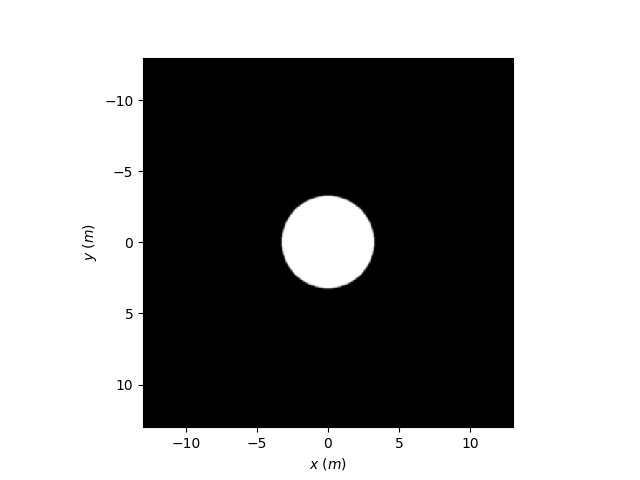
\includegraphics[scale=0.45]{simplepupil.png}
  \caption{The simplest pupil function, a circle}\label{fig:simplepupil}
\end{figure}

The reality of the discreteness of computers presents a problem when considering this simple pupil. Since the pixel luminance value is either 0 or 1 in the function, the edges of the circle are jagged. This produces FFT alias artifacts in the PSF, damaging our data. To resolve this, we used a Gaussian filter with standard deviation $\sigma = 1$; this filtering is shown in Fig.~\ref{fig:simplepupil} with the soft edges on the circle. Furthermore, to ensure that the FFT would not cause aliasing issues, we padded our image with $\sim$1 diameter of the aperture on either side; a padding scale of $1.183$ diameters had the best results overall for each PSF\@.

Analytically, the Fourier transform of this pupil function is an example of the 2D polar Fourier transform. Generally, the 2D Fourier transform is of the form:
\begin{equation}
  F(k_x, k_y) = \frac{1}{2\pi}\int\D A\ f(x, y)\exp\left[-\iu(k_x x + k_y y)\right] \label{eq:2dfourier}
\end{equation}
If we perform these transformations:
\begin{align*}
  x &= r\cos\phi & k_x &= k\cos\psi \\
  y &= r\sin\phi & k_y &= k\sin\psi
\end{align*}
then the 2D Fourier transform turns into:
\begin{equation}
  F(k, \psi) = \frac{1}{2\pi}\int\D A\ f(r, \phi)\exp\left[-\iu kr(\cos(\phi - \psi))\right] \label{eq:2dpolarfourier}
\end{equation}
In the special situation where the function $f$ has rotational symmetry, i.e. $f=f(r)$, the integral simplifies to a 1D integral in $r$:
\begin{equation}
  F(k) = \int_0^{\infty}\D r\ r f(r)J_0(kr) \label{eq:2dpolarfouriersym}
\end{equation}
where $J_0$ is the zeroth order of the Bessel function of the first kind. This is the particular integral we care about; the circular aperture obviously has rotational symmetry and has well defined limits: 0 to $R$. Therefore, this integral evaluates to
\begin{equation*}
  F(k) = \frac{R}{k}J_1(R k)
\end{equation*}
However, since the luminance information in an image is only characterized by the intensity, we must take the square of this function to find the desired PSF\@:
\begin{equation}
  PSF_{\text{simp}}(k) = R^2 \left(\frac{J_1(R k)}{k}\right)^2 \label{eq:psf-simp}
\end{equation}
This particular function generates the \textit{Airy pattern}, a set of concentric circles decaying in luminosity.

\begin{figure}[!ht]
  \centering
    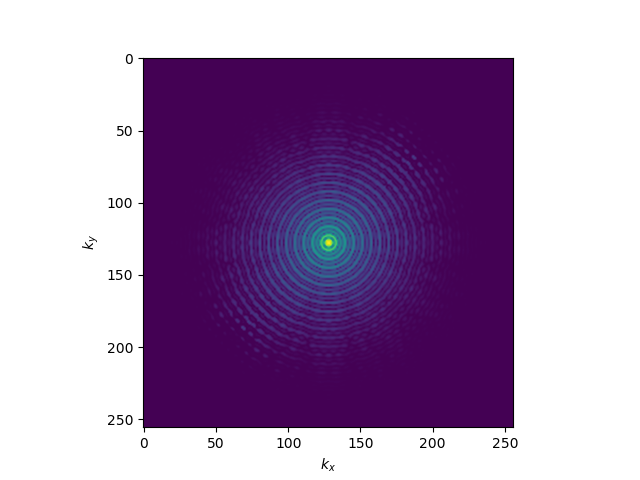
\includegraphics[scale=.45]{simplepsf.png}
  \caption{The computed PSF of the circular aperture}\label{fig:simplepsf}
\end{figure}

Using $N=256$ samples per each axis ($x$ and $y$), we performed an FFT on the Gaussian-filtered circular pupil function which produced the image in Fig.~\ref{fig:simplepsf}. The ringing and decaying pattern matches what we expected from the theoretical model!

\subsection{Cassegrain Aperture}\label{subsec:cassegrain-aperture}
[Cassegrain aperture is basically a superposition of Bessel functions; prove and show]

\subsection{Actual Telescope Construction}\label{subsec:actual-aperture}
[Include discussion of struts and the Hubble Telescope]

\section{The Effects of Environmental Factors on the Point Spread Function}\label{sec:environment}

The phase shift in the complex pupil function (Eq.~\ref{eq:pupilFunc}) can arise from different environmental factors such as imperfections in the telescope mirror or light-particle interactions in the atmosphere. To analyze how these factors affect the PSF, we simulate the phase shifts using Gaussian random fields scaled by different power spectra corresponding to the different factors.


\subsection{Gaussian Random Field Simulation}\label{subsec:gaussian-fields}
In order to simulate phase shifts from different causes, we have created a function that will generate a Gaussian random field given a power spectrum, $P(k)$. The values in the fields are selected from Gaussian distributions with a mean of zero and a scaling determined by the power spectrum. They are created by selecting an independent Gaussian random value for each Fourier mode in $\vec{k}-$space followed by an inverse FFT back to configuration space. An example of one such field is shown in Figuret\ref{fig:GaussianRandField}

\begin{figure}[h!]
  \centering
    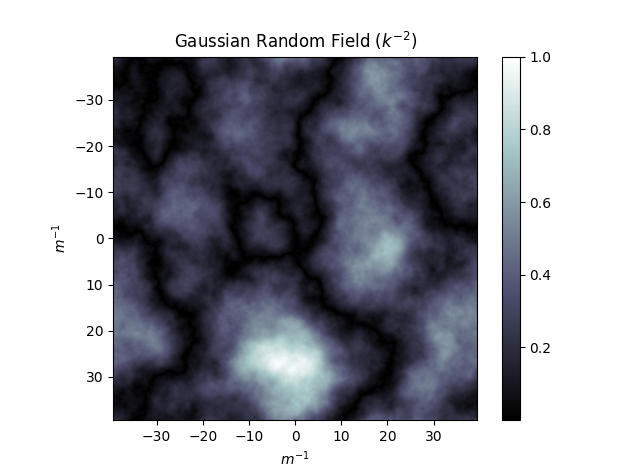
\includegraphics[scale=.45]{gaussrandfield.png}
  \caption{Gaussian Random Field Simulation}\label{fig:GaussianRandField}
\end{figure}

\subsection{Mirror Imperfections}\label{subsec:mirror-issues}
Small imperfections in the mirror can produce phase shifts of correspondingly small wavelengths and will therefore be simulated by passing a $P(k)$ with power at large $k$ into our Gaussian random field generating function.

[Include discussion and verification of when these shifts become a major problem]

\subsection{Atmospheric Fluctuations}\label{subsec:atmosphere-model}

[Include field modeling to demonstrate how the atmosphere affects ground-based telescopes]

\section{Bibliography}\label{sec:references}

}\end{document}
